\section{Synthetic Validation}\label{sec:synthetic}

Before turning to real data, we verify that the crossover characterized in \Cref{sec:theory} materializes under stochastic-gradient training on finite samples, using a data-generating process (DGP) whose exogenous level predictability is known exactly.

\paragraph{Data-generating process}
Covariates follow an AR(1) process, $x_t = 0.9\,x_{t-1} + \epsilon_t$ with $\epsilon_t \sim \mathcal{N}(0,1)$. The series level mixes an exogenously explained component and a covariate-orthogonal random walk,
\[
m_t \;=\; \sqrt{\lambda}\,\beta^\top \tilde{x}_t \;+\; \sqrt{1-\lambda}\,u_t,
\qquad u_t = u_{t-1} + \eta_t,\;\; \eta_t \sim \mathcal{N}(0,\sigma_u^2),
\]
where $\tilde{x}_t$ denotes standardized covariates, so that by construction the population $R^2$ of the level regression equals $\lambda$ (we verify this identity empirically on each generated series). The observed series adds a shape component with daily seasonality, $z_t = A\sin(2\pi t/P) + \rho\,z_{t-1} + \nu_t$ with period $P=24$, giving $y_t = m_t + \sigma_0 z_t$. Thus $\lambda$ is a direct, controllable analogue of the $\lps$ diagnostic of \Cref{sec:lps}.

\paragraph{Sweep design}
We sweep $\lambda \in \{0.0, 0.1, \dots, 1.0\}$ (11 points), horizons $h \in \{24, 96, 336\}$, lookbacks $L \in \{96, 336\}$, ten seeds, and four normalization arms---\rawm{} (global z-score only), RevIN \citep{kim2022revin}, \cnm-oracle (true $m_t$), and \cnm-est (LightGBM first stage \citep{ke2017lightgbm})---for $11 \times 3 \times 2 \times 10 \times 4 = 2{,}640$ runs. Each series has length 20{,}000 with a chronological 6:2:2 train/validation/test split. The backbone is fixed to RLinear \citep{li2023rlinear} in every arm: because the theory of \Cref{sec:theory} is linear-Gaussian, the validation experiment must use a backbone in exactly that function class---a theory--experiment fidelity principle we maintain throughout (capacity is never a confound; only the normalization varies across arms). Nonlinear backbones enter only in the real-data study of \Cref{sec:empirical}.

\paragraph{Gate~1 results}
The experiment was pre-registered as a go/no-go gate with three criteria; all three passed. \Cref{fig:synth} overlays the empirical seed-mean $\mse$ points on the closed-form constrained-OLS theory curves.

\emph{(i) Crossover location.} The empirical IN/CN crossing $\lamstar_{\mathrm{emp}}$ matches the constrained-OLS prediction in all six $(h,L)$ cells, with maximum absolute deviation $0.015$ (criterion: $\pm 0.1$). At $L=96$ the (empirical, theory) pairs are $(0.009, 0.007)$, $(0.011, 0.009)$, and $(0.022, 0.022)$ for $h = 24, 96, 336$; at $L=336$ they are $(0.018, 0.007)$, $(0.023, 0.008)$, and $(0.029, 0.021)$.

\emph{(ii) Horizon monotonicity.} As predicted by \Cref{sec:theory}, the IN--CN gap at fixed $\lambda = 0.8$ widens with $h$: seed-paired increments are $+0.1699 \pm 0.0336$ ($h{=}24 \to 96$) and $+0.0314 \pm 0.0244$ ($h{=}96 \to 336$) at $L=96$, and $+0.1276 \pm 0.0193$ and $+0.0395 \pm 0.0158$ at $L=336$ (95\% confidence intervals).

\emph{(iii) First-stage error.} The degradation of \cnm-est relative to \cnm-oracle is explained by the measured first-stage error $\sest$ inserted into the theory: the median experiment-to-theory degradation ratio is $1.12$, well inside the pre-registered $[0.5, 2.0]$ band.

\paragraph{A discrepancy that sharpens the theory}
The stylized restoration-rule model M1 predicts $\lamstar_{\mathrm{M1}} \approx 0.27$--$0.28$ at these settings, yet the observed crossings lie at $0.009$--$0.029$. The resolution is Proposition~2$'$ (\Cref{sec:theory}): a linear backbone applied to instance- or globally-normalized inputs implicitly performs OLS-style tracking of residual level drift inside the lookback window, so the operative \rawm{} and \cnm{} estimators are strictly stronger than M1's pure restoration rules \citep{toner2024linear}. The constrained-OLS curves---the exact optima within each normalization's function class---capture this and match the experiments; $\lamstar_{\mathrm{M1}}$ is an upper bound, and the $\lamstar_{\mathrm{M1}} - \lamstar_{\mathrm{OLS}}$ gap measures the size of implicit level tracking. The practical implication is notable: when no covariate-orthogonal drift separates train and test ($\sdel = 0$), \cnm{} dominates from very small $\lambda$ onward. Instance normalization's practical niche is therefore drift robustness---precisely the distribution-shift setting that motivated RevIN---rather than level prediction per se, a point we revisit on real data in \Cref{sec:empirical}.

\begin{figure}[t]
  \centering
  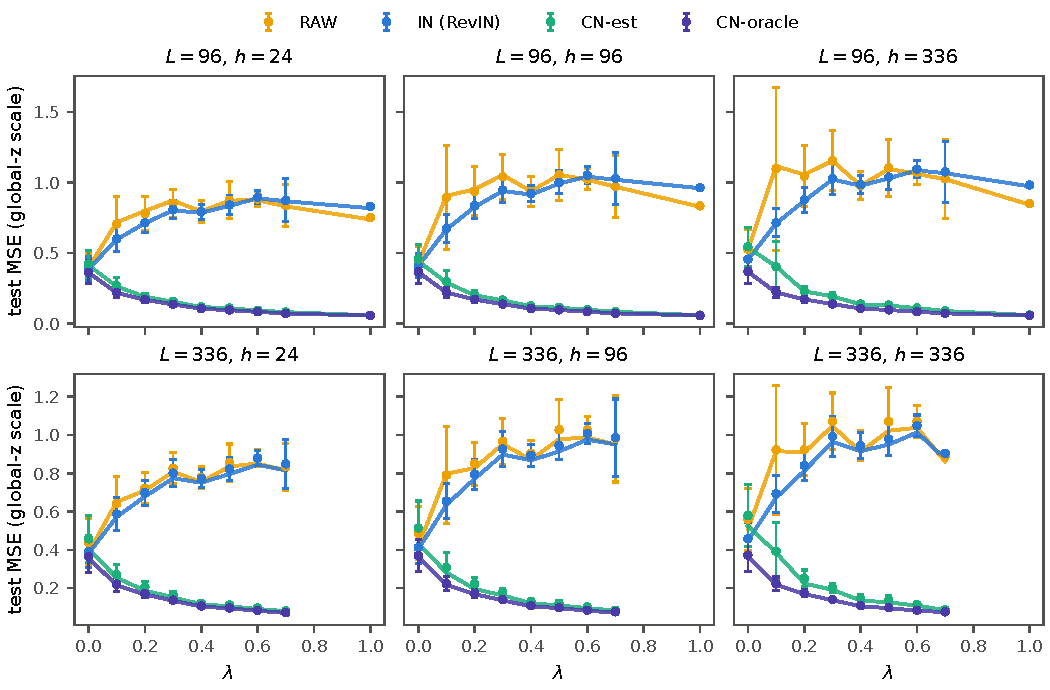
\includegraphics[width=\textwidth]{figures/fig2_synth.pdf}
  \caption{Synthetic validation (Gate~1). Empirical seed-mean test $\mse$ (points, $\pm$1 s.d.\ across ten seeds) overlaid on closed-form constrained-OLS theory curves (lines) for \rawm, RevIN, \cnm-oracle, and \cnm-est as a function of the exogenous level-predictability share $\lambda$, across horizons $h \in \{24, 96, 336\}$ and lookbacks $L \in \{96, 336\}$. Empirical IN/CN crossings match theory within $0.015$; the gap at high $\lambda$ widens with $h$.}
  \label{fig:synth}
\end{figure}
